\section{Preliminaries}\label{sec:prelim}
A planned cyber attack on the SCADA system takes place through multiple steps in which the software protection elements are compromised. This entire process can be effectively modeled using attack trees. A cyber intrusion consists of vulnerabilities in the cyber system and the dependency among them to be exploited. Therefore, a cyber attack can be represented as a directed graph with vulnerabilities denoted by the nodes and edges symbolizing the dependencies. In this section, the attack tree representation of a cyber attack on the SCADA system and the method to evaluate probability of successful intrusion are detailed.
\subsection{Attack Tree Representation of Vulnerabilities}
In this paper, the attack graph $\mathcal{G}(\mathcal{V}\bigcup\mathcal{C})$ consists of two types of nodes: exploit to vulnerabilities denoted by $\mathcal{V}$ and conditions required for exploiting represented as $\mathcal{C}$. The preconditions needed to exploit a vulnerability are assumed to be either initial conditions of the attack or resulting output of some previously occurred exploit. In this case, three preconditions are required to be satisfied in order to exploit a vulnerability: (\textit{i})service which is denoted by \emph{Service Name}(\emph{Source Host ID}), (\textit{ii})connection represented by $\langle$\emph{Source Host ID},\emph{Target Host ID}$\rangle$ and (\textit{iii})privilege which is denoted as \emph{Privilege Name}(\emph{Source Host ID}).

For example, a cyber intrusion scenario is considered for a control center SCADA system, where an adversary aims to gain unauthorized access to control assets in the power system. The cyber intruder has to access the application server for this purpose which is dedicated to send control commands to open/close circuit breakers in the power system. In order to do so, the adversary needs to gain access of the historian server through a firewall and thereafter reach the application server through a different firewall as shown in Fig.~\ref{fig:example}.
\begin{figure}[htbp]
	\centering
	
\includegraphics[scale=0.4]{fig-example.png}
	\caption{Cyber intrusion scenario in control center application server.}
	\label{fig:example}
\end{figure}

Let there be two possible exploits to the vulnerabilities in the first firewall denoted by $\langle\textrm{Ser}1,0,1\rangle$ and $\langle\textrm{Ser}2,0,1\rangle$ as shown in Fig.~\ref{fig:attacktree}. The first one is assumed to be a zero day exploit and the second one is considered as a known exploitation. A zero day exploit to a vulnerability is one which may not be publicly known but identified by an intruder. In order to exploit either of the vulnerabilities, the intruder needs the privilege \emph{user}(\emph{0}) (which denotes him being present) and is required to be connected to the historian server through $\langle$\emph{0},\emph{1}$\rangle$. Additionally, the vulnerabilities require the services \emph{Ser1(1)} and \emph{Ser2(1)} respectively to be available for them to be exploited. Once the vulnerability is successfully exploited, the intruder gains the user privilege \emph{user}(\emph{1}) of the historian server. This output of previously occurred exploit can be used as a precondition of the successive exploits. Let there be a single zero-day exploit to a vulnerability in the second firewall denoted by $\langle\textrm{Ser}3,1,2\rangle$. This can be successfully exploited by an intruder having privilege \emph{user}(\emph{1}) to obtain access to the application server. Thereafter, the intruder can utilize the privilege \emph{user}(\emph{2}) of the application server to reach the goal privilege \emph{root}(\emph{2}).
\begin{figure}[htbp]
	\centering
	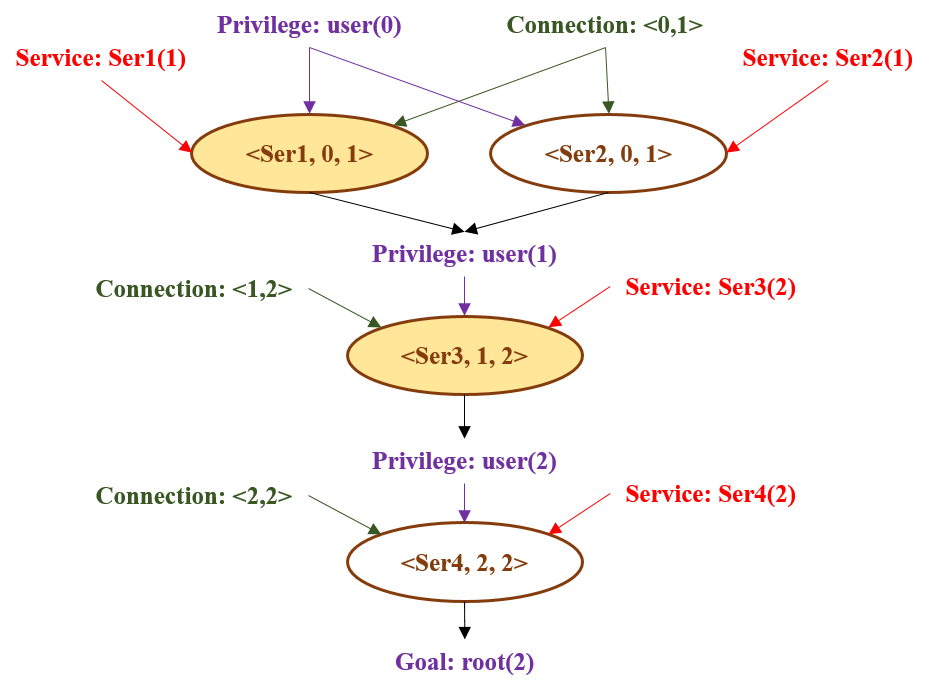
\includegraphics[scale=0.4]{fig-attacktree.png}
	\caption{Attack tree representation of cyber intrusion in control center application server.}
	\label{fig:attacktree}
\end{figure}
\subsection{Modeling Bayesian Attack Tree}
Attack trees can be effectively modeled using Bayesian networks (BN) which are widely used to develop the probabilistic model for the same. BN is denoted by a pair $\langle\mathcal{G},\mathcal{N}\rangle$ where $\mathcal{G}(\mathcal{V},\mathcal{E})$ denotes a directed graph and $\mathcal{N}$ represents a set of parameters. In a BN, the probability of each node is dependent on the conditional probability of its parent nodes defined on the parameters in $\mathcal{N}$. The above attack tree is modeled as a Bayesian attack tree to evaluate the probability of a successful intrusion to the target condition. For this purpose, the individual probability of a successful exploitation of a vulnerability is required to be calculated. Every vulnerability can be scored based on its severity of being exploited by a standard Common Vulnerability Scoring System (CVSS)~\cite{cvss}. Since the scores are provided on a scale from $0$ to $10$, they can be normalized through division by $10$. The probability of a successful exploit on a vulnerability ($v_i$) with preconditions satisfied is given by
\begin{equation}
\mathbb{P}(v_i|s_i,l_i)=\dfrac{\mathsf{CVSS}(v_i)}{10}
\end{equation}
where $s_i$ and $l_i$ respectively denote that the service and connection required to exploit the vulnerability $v_i$ are available. For known vulnerabilities, the CVSS scores can be evaluated from~\cite{nist1,nist2} depending on the level of access complexity, authentication requirements and other factors. The CVSS score for the zero-day exploits are evaluated as $0.8$ if the severity of access complexity and authentication requirements is considered to be the highest. 

Thereafter, using the Bayes' theorem, the probability  of a successful exploit on a vulnerability ($v_i$) is calculated as
\begin{equation}
\mathbb{P}(v_i)=\mathbb{P}(s_i)\cdot\mathbb{P}(l_i)\cdot\dfrac{\mathsf{CVSS}(v_i)}{10}
\end{equation}
The probabilities of availability of service and connection given by $\mathbb{P}(s_i)$ and $\mathbb{P}(l_i)$ respectively can be randomly selected from $0.85$ to $1.0$. The initial probability of availability of user privilege $\mathbb{P}(c_i)$ is considered to be $1.0$ since it is assumed that the intruder is present to perform the cyber attack. For evaluating the availability of privileges in the successive target vulnerabilities, the probability of a successful intrusion through the preceding vulnerability is calculated. Therefore, the attack tree follows the structure of a \textit{Markov Chain} where the probability of occurrence of a state is only dependent on the probability of occurrence of preceding state(s). 

Certain access privileges can be achieved by exploiting more than one vulnerability from multiple prior access privileges. The probability of successfully reaching the condition $c_i$ from $n$ privileges ($c_j,j=1,2,\cdots n$) through the $m_j$ vulnerabilities $v_k,k=1,2,\cdots m_j$ is given by
\begin{equation}
\mathbb{P}(c_i)=\sum_{j=1}^{n}{\mathbb{P}\bigg(\bigcup_{k=1}^{m_j}v_k\bigg)\mathbb{P}(c_j)}
\end{equation} 
Finally the probability of successfully exploiting a target vulnerability through a minimal attack sequence is considered. It is assumed that the adversary does not waste any time in attacking multiple vulnerabilities of the same system while targeting a given goal condition. In order to calculate this probability, a backward traversal is considered from the target condition ($c_i$) to each of the possible vulnerabilities $v_j$. The probability of successful intrusion through each $v_j$ to reach target $c_i$ is given by
\begin{equation}
\mathbb{P}(v_j\wedge c_i)=
\begin{cases}
\mathbb{P}(v_j)\cdot\mathbb{P}(c_i|v_j), &j=1\\
\mathbb{P}(v_j)\cdot\prod_{k\neq j}\mathbb{P}(v_k=False), &j>1\\
\quad\cdot\mathbb{P}(c_i|v_j=True,v_{k\neq j}=False) &
\end{cases}
\end{equation}